\documentclass[a4paper,11pt]{report}
\usepackage[T1]{fontenc}
\usepackage[utf8]{inputenc}
\usepackage[polish]{babel}
\usepackage{lmodern}
\usepackage{graphicx}
\usepackage{geometry}

\title{Różne przypadki złożoności obliczeniowej algorytmu Quicksort}
\author{Monika Litwin 200586}
\begin{document}
\maketitle

\begin{figure}
  \begin{center}
  \textbf{Trochę teorii}
\\
\begin{flushleft}\underline{Przypadek optymistyczny}\end{flushleft}
Teoretycznie takowy występuje, gdy sortowany jest już uporządkowany zbiór \\(z niewielką ilością elementów nie na swoich miejscach). \\Wtedy złożoność wynosi \emph{O(nlogn)}

\begin{flushleft}\underline{Przypadek typowy}\end{flushleft}
Zbiór poddany algorytmowi sortowania posiada losowo rozłożone elementy.\\ Złożoność wynosi \emph{O(2nlogn)}

\begin{flushleft}\underline{Przypadek pesymistyczny}\end{flushleft}
Występuje dla zbiorów o elementach posortowanych odwrotnie.\\ Złożoność wynosi \emph{O($\frac {n^{2}}{2}$)}

    \label{fig:}
  \end{center}
\end{figure}

\begin{figure}
  \begin{center}
	\textbf{Sortowanie zbioru odwrotnie posortowanych elementów}
\\ Poniżej zamieszczony jest wykres pomiarów czasu dla algorytmu, któremu podano wcześniej posortowany w odwrotnej kolejności wektor. 
W testach mojego algorytmu sortowania Quick, najszybszy okazał się właśnie ten przypadek.

    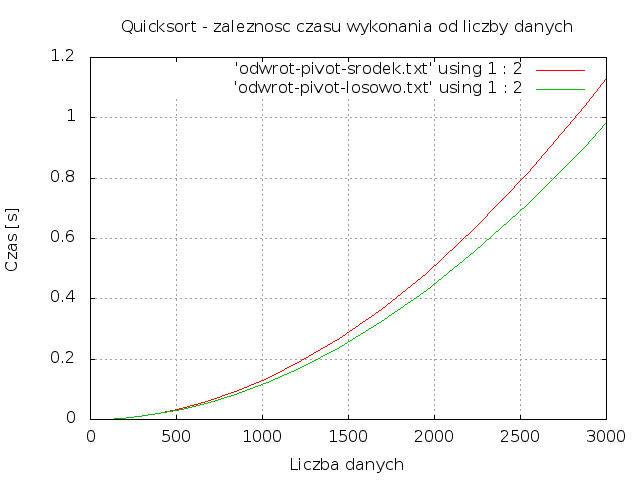
\includegraphics[scale=0.5]{./odwrotnie.png}
    \label{fig:}
  \end{center}
\end{figure}

\begin{figure}
  \begin{center}
  \textbf{Sortowanie zbioru posortowanych elementów}
\\Kolejnym jeśli chodzi o szybkość wykonania okazał się być algorytm, w którym sortujemy posortowany już wektor. Jego czas wykonania nie różni się znacznie od wcześniejszego przypadku.
\\
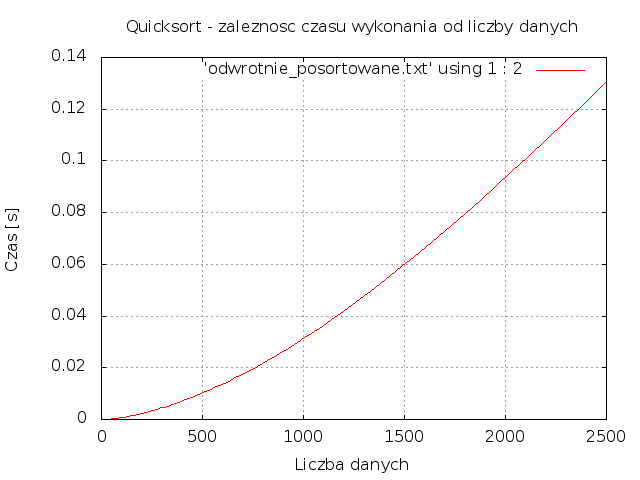
\includegraphics[scale=0.5]{./posortowane.png}
  \end{center}
\end{figure}

\begin{figure}
  \begin{center}
  \textbf{Sortowanie zbioru rozłożonych losowo elementów}
\\
Jeszcze wolniej wykonuje się nasz algorytm Quicksort, gdy podamy do niego wektor z nieuporządkowanymi elementami. Jednak również jest to niewielkie odchylenie w stosunku do wcześniejszych przypadków.

    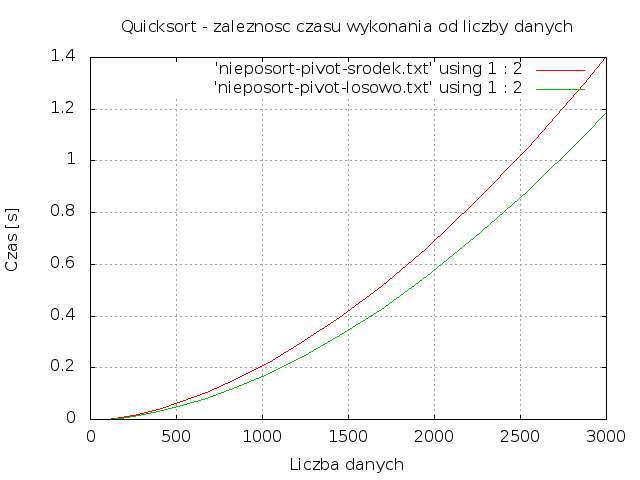
\includegraphics[scale=0.5]{./nieposotrowane.png}
    \label{fig:}
  \end{center}
\end{figure}

\begin{figure}
  \begin{center}
  \textbf{Sortowanie zbioru nieuporządkowanego z losowo wybieranym pivotem}
  \\W testach ten przypadek sortowania szybkiego wypadł zdecydowanie najgorzej. Okazał się stanowczo najwolniejszy. Znacząco odbiega swoją złożonością od wcześniej prezentowanych. 
  \\
  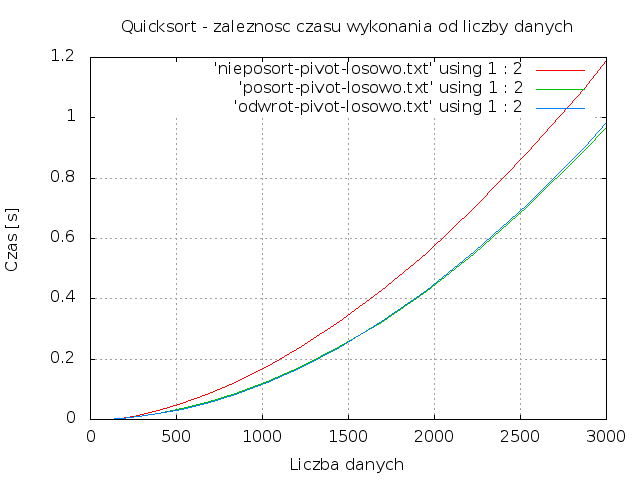
\includegraphics[scale=0.5]{./pivot-losowo.png}
    \label{fig:}
  \end{center}
\end{figure}

\begin{figure}
  \begin{center}
  \textbf{Porównanie wszystkich przypadków}
  \\
Po testach okazało się, że teoria niewiele ma wspólnego z otrzymanymi wynikami pomiarów. Sortowanie odwrotnie posortowanych elementów - przypadek, który miał być najwolniejszy okazał się najszybszy. Algorytm, do którego podawałam prawidłowo posortowane dane plasuje się pośrodku, zamiast, zgodnie z przypuszczeniami - na czele. Najwolniejszy, i to bardzo wyraźnie, jest przypadek, gdzie element osiowy wybierany był losowo, co według założeń miało usprawnić działanie algorytmu, zmniejszając prawdopodobieństwo wystąpienia opcji pesymistycznej.
Wynika to prawdopodobnie z różnic w sposobie implementacji algorytmu Quicksort, przyjętego sposobu mierzenia czasu lub ewentualnego błędu w trakcie przeprowadzania pomiarów. 
\\
    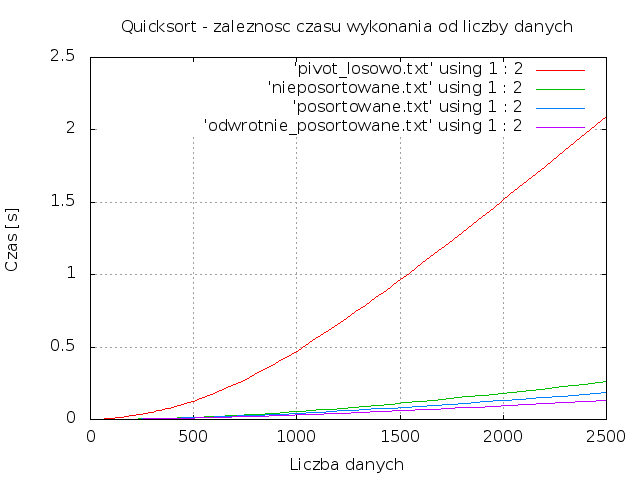
\includegraphics[scale=0.5]{./quickRazem.png}
    \label{fig:}
  \end{center}
\end{figure}

\end{document}
